\section{Control Architecture}

\begin{frame}{Control scheme}
	\begin{figure}
		\centering
		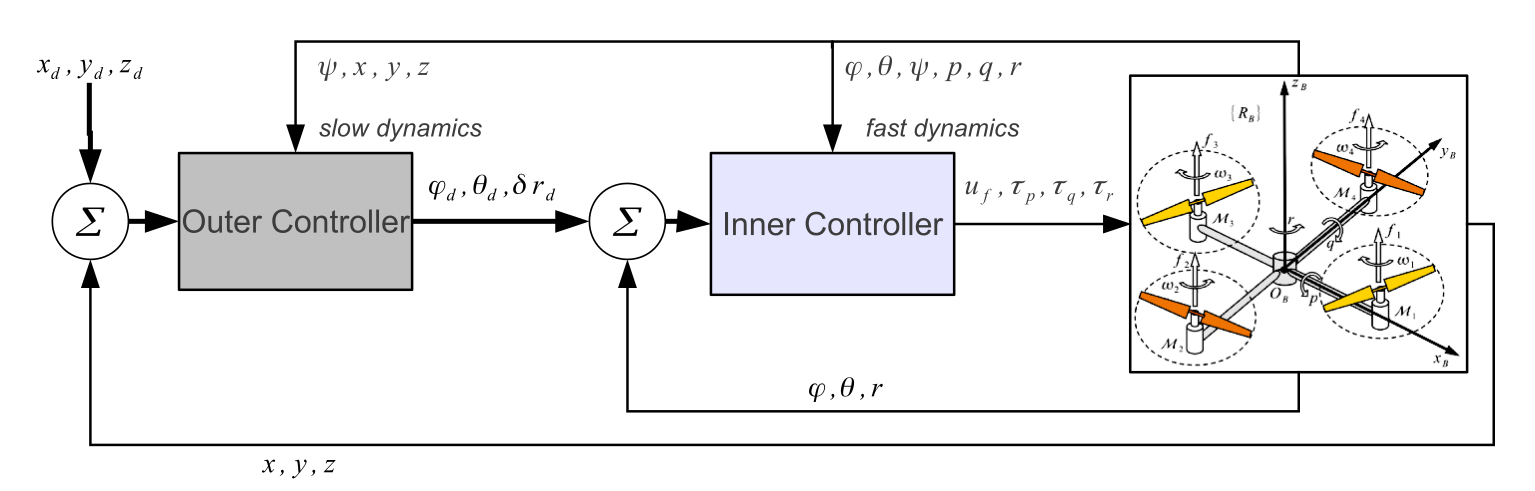
\includegraphics[width=1.0\linewidth]{Images/ControlScheme}
		\caption{The double loop architecture in case of actuator loss.}
		\label{fig:controlscheme}
	\end{figure}
\end{frame}

\subsection{Quadrotor model in case of rotor loss}

\begin{frame}{Generalized force - real actuation mapping}
	
	In case of failure of rotor $ \mathcal{M}_2 $ the mapping \eqref{force_mapping} is:
	\begin{equation}
	\begin{bmatrix}
	u_f \\ \tau_q \\ \tau_r
	\end{bmatrix} = 
	\begin{bmatrix}
	1 & 1 & 1 \\
	-l & l & 0 \\
	d  & d & -d
	\end{bmatrix}
	\begin{bmatrix}
	f_1 \\ f_3 \\ f_4
	\end{bmatrix}
	\label{forceTorqueMappingFailure}
	\end{equation}
	and the neglected input is $ \tau_p = l \cdot f_4 $
	\pause
	
	The inverse of \eqref{forceTorqueMappingFailure} is:
	\begin{equation}
	\begin{bmatrix}
	f_1 \\ f_3 \\ f_4
	\end{bmatrix} = \frac{1}{4} 
	\begin{bmatrix}
	1 & -2/l & l/d \\
	1 & 2/l & l/d \\
	2 & 0 & -2/d
	\end{bmatrix}
	\begin{bmatrix}
	u_f \\ \tau_q \\ \tau_r
	\end{bmatrix}
	\end{equation}
	
\end{frame}

\begin{frame}{State-space model}
	
	\begin{block}{State vector}
		\begin{align*}
		\mathbf{x} \ &= \ [&x_1 &\ &x_2 &\ &x_3 &\ &x_4 &\ &x_5 &\ &x_6 &\ &x_7 &\ &x_8 &\ &x_9 &\ &x_{10} &\ &x_{11} &\ &x_{12} \ ]^T \\
		&= \ [&\phi &\ &\theta &\ &\psi &\ &p &\ &q &\ &r &\ &x &\ &y &\ &z &\ &\dot{x} &\ &\dot{y} &\ &\dot{z} \ ]^T
		\end{align*}
	\end{block}
	\begin{block}{Input vector}
		\begin{equation}
		\mathbf{u} \ = \ [ \ u_1 \quad u_2 \quad u_3 \ ]^T \ = \ [ \ u_f \quad \tau_q \quad \tau_r \ ]^T
		\end{equation}
	\end{block}
	
	The neglected input is expressed as:
	\begin{equation}
		\tau_p = \dfrac{l}{2}(u_1- \dfrac{u_3}{d})
	\end{equation}

\end{frame}

\begin{frame}{State-space model}
	\begin{equation}
		\begin{cases}
		\dot{\phi} & = \dot{x}_1 = x_4 + x_5 S_{x_1} T_{x_2} + x_6 C_{x_1} T_{x_2} \\
		\dot{\theta} & = \dot{x}_2 = x_5 C_{x_1} \\
		\dot{\psi} & =  \dot{x}_3 = \frac{1}{C_{x_2}} [ x_5 S_{x_1} + x_6 C_{x_1}] \\
		\dot{p} & = \dot{x}_4 = \frac{1}{I_{xx}}[-k_r x_4 - x_5 x_6 (I_{zz} - I_{xx}) + \frac{l}{2} (u_1 -\frac{u_3}{d})] \\
		\dot{q} & = \dot{x}_5 = \frac{1}{I_{xx}}[-k_r x_4 - x_5 x_6 (I_{zz} - I_{xx}) + u_2]\\
		\dot{r} & = \dot{x}_6 = \frac{1}{I_{xx}}(-k_r x_6 + u_3) \\
		\dot{x} & = \dot{x}_7 = x_{10} \\
		\dot{y} & = \dot{x}_8 = x_{11} \\
		\dot{z} & = \dot{x}_9 = x_{12} \\
		\ddot{x} & = \dot{x}_{10} = \frac{C_{x_1} S_{x_2} C_{x_3} + S_{x_1} S_{x_3}}{m} u_1 - \frac{k_t}{m}x_{10} \\
		\ddot{y} & = \dot{x}_{11} = \frac{C_{x_1} S_{x_2} S_{x_3} - S_{x_1} C_{x_3}}{m} u_1 - \frac{k_t}{m}x_{11} \\
		\ddot{z} & = \dot{x}_{12} = \frac{1}{m} [u_1 C_{x_1} C_{x_2} - k_t x_{12} - m g]
		\end{cases}
		\label{completeQuadModel}
	\end{equation}
\end{frame}

\section*{Outer control loop}

\begin{frame}{Outer control loop}
	The horizontal motion depends on the projection of the thrust vector on the $ (x,y) $ plane.
	
	The direction of this vector depends on the roll and pitch angles.
	\bigskip
	\begin{alertblock}{Task of the Outer control: \bigskip}
		Generate the right values of:
		\begin{itemize}
			\item roll and pitch angles to reach a desired horizontal position;
			\item yaw velocity to control vertical dynamics.
		\end{itemize} 
	\end{alertblock}
\end{frame}

\begin{frame}{Outer control loop}
	
	Assuming the inner control loop stabilizes the state near the equilibrium:
	
	\begin{equation}
	x_1=\phi \rightarrow \phi_d, \qquad x_2=\theta \rightarrow \theta_d, \qquad x_6=r \rightarrow r_d
	\end{equation}
	\bigskip
	
	\begin{block}{Inputs at the steady-state are: }
		\begin{align*}
			u_2& \rightarrow 0 \\
			u_3& \rightarrow x_{6d} k_r \\
			u_1& \rightarrow \dfrac{u_3}{d}= \dfrac{x_{6d} k_r}{d}
		\end{align*}
	\end{block}

\end{frame}

\begin{frame}{Outer control loop}
	Rewrite the equations relative to $ (x,y,z) $ dynamics of \eqref{completeQuadModel} using:
	\begin{enumerate}
		\item assumption of small angles for $ \phi_d $ and $ \theta_d $
		\item inputs written at the steady-state
		\item \textit{new} state for outer control loop:
		\begin{align*}
		\tilde{x} \ &= \ [ \ \tilde{x}_1 \quad \tilde{x}_2 \quad \tilde{x}_3 \quad \tilde{x}_4 \quad \tilde{x}_5 \quad \tilde{x}_6 \ ]^T \\
		&= \ [ \ x_7 \quad x_8 \quad x_9 \quad x_{10} \quad x_{11} \quad x_{12} \ ]^T
		\end{align*}
		\item \textit{new} control inputs vector:
		\begin{equation}
		\tilde{u} = [\tilde{u}_1 \quad \tilde{u}_2 \quad \tilde{u}_3] = \Big[ \dfrac{k_r x_{6d}}{dm}  x_{1d} \quad  \dfrac{k_r x_{6d} }{dm} x_{2d} \quad  \dfrac{k_r x_{6d}}{dm} \Big]
		\label{OuterInputs}
		\end{equation}
	\end{enumerate}

\end{frame}

\begin{frame}{Outer control loop}
	\begin{alertblock}{Outer control loop model:}
		\begin{align*}
		\dot{\tilde{x}}_1 & = \tilde{x}_4 \\
		\dot{\tilde{x}}_2 & = \tilde{x}_5 \\
		\dot{\tilde{x}}_3 & = \tilde{x}_6 \\
		\dot{\tilde{x}}_4 & = C_\psi \tilde{u}_2 + S_\psi \tilde{u}_1 - \dfrac{k_t}{m} \tilde{x}_4 \\
		\dot{\tilde{x}}_5 & = S_\psi \tilde{u}_2 - C_\psi \tilde{u}_1 - \dfrac{k_t}{m} \tilde{x}_5 \\
		\dot{\tilde{x}}_6 & = \tilde{u}_3 - \dfrac{k_t}{m} \tilde{x}_6 - g
		\label{outerControl_}
		\end{align*}		
	\end{alertblock}
	\pause
	\centering
	\Ovalbox{\textbf{Not yet linear!}}
\end{frame}

\begin{frame}{Outer control loop}
	To linearize the nonlinear dynamics we manipulate the control inputs:
	\begin{equation}
	\begin{bmatrix}
	\tilde{u}_1 \\ \tilde{u}_2
	\end{bmatrix} = 
	\begin{bmatrix}
	S_{\psi} & -C_{\psi} \\
	C_{\psi} & S_{\psi} 
	\end{bmatrix}
	\begin{bmatrix}
	\tilde{\tilde{u}}_1 \\ \tilde{\tilde{u}}_2
	\end{bmatrix}
	\label{rotation_matrix_outer}
	\end{equation}
	
	Obtaining:
	\begin{align*}
	\dot{\tilde{x}}_4 & = \tilde{\tilde{u}}_1 - \dfrac{k_t}{m} \tilde{x}_4 \\
	\dot{\tilde{x}}_5 & = \tilde{\tilde{u}}_2 - \dfrac{k_t}{m} \tilde{x}_5 \\
	\dot{\tilde{x}}_6 & = \tilde{u}_3 - \dfrac{k_t}{m} \tilde{x}_6 - g
	\end{align*}
	\pause
	\centering
	\Ovalbox{\textbf{Linear and decoupled}}
\end{frame}

\begin{frame}{Outer control loop}
	The control inputs are chosen as:
	\begin{equation}
	u_i = \ddot{x}_i + 2\xi_{out}c_{out} \dot{e}_i + c_{out}^2 e_i 
	\end{equation}
	where:
	\begin{itemize}
		\item $ \ddot{x}_i $ is the feed-forward term;
		\item $ e_i = x_{di} - x_i $ is the error;
		\item $ c_{out} $ represents the natural frequency of the system and must be small: we want the outer loop control to be slower then inner control loop;
		\item $ \xi_{out} $ represents the dumping of the system.
	\end{itemize}
\end{frame}

\section*{Inner control loop}

\begin{frame}{Inner control loop}
	\begin{alertblock}{Task of Inner control loop: }
		\bigskip \hfill to control the dynamics of the attitude angle and the yaw velocity.
	\end{alertblock}
	\bigskip
	Equation relative to $ \psi, \theta, p, q, r $ expressed such that the origin of the system is an equilibrium point when the inputs are equal to zero.
	
	\begin{block}{State vector:}
		\begin{equation}
		\hat{x} = [ \ \hat{x}_1 \quad \hat{x}_2 \quad \hat{x}_3 \quad \hat{x}_4 \quad \hat{x}_5 \ ] = \Big[ \ x_1 \quad x_1 \quad x_2 \quad x_3 \quad x_4 \quad (x_6-\dfrac{mgd}{k_r}) \ \Big]	
		\end{equation}
	\end{block}

	\begin{block}{Inputs vector:}
		\begin{equation}
		\hat{u} = [ \ \hat{u}_1 \quad \hat{u}_2 \quad \hat{u}_3 \ ] = [ \ (u_1 -mg) \quad u_2 \quad (u_3 - mgd) \ ]
		\end{equation}
	\end{block}
\end{frame}

\begin{frame}{Nonlinear model}
	The system is described by:
	\begin{align}
		&{\dot{\hat{x}} \ =  \ \hat{f} \ (\hat{x}) \ + \ \hat{G} \ (\hat{x}) \ \hat{u}} \\
		&{\hat{y}}  =  [ \ \hat{h}_1 \quad \hat{h}_2 \quad \hat{h}_3 \ ] = [ \ \hat{x}_1 \quad \hat{x}_2 \quad \hat{x}_5 \ ]
	\end{align}
	where:
	\begin{columns}
	\column{0.55\textwidth}
	\begin{equation*}
	\hat{f}(\hat{x})=
	\begin{bmatrix}
	\hat{x}_3 + \hat{x}_4 S_{\hat{x}_1} T_{\hat{x}_2} + (\hat{x}_5 + \dfrac{mgd}{k_r}) C_{\hat{x}_1} T_{\hat{x}_2} \\
	\hat{x}_4 C_{\hat{x}_1} - (\hat{x}_5 + \dfrac{mgd}{k_r}) s_{\hat{x}_1}  \\
	\dfrac{1}{I_{xx}} [-k_r \hat{x}_3 - \hat{x}_4(\hat{x}_5 + \dfrac{mgd}{k_r}) (I_{zz} - I_{yy}) ] \\
	\dfrac{1}{I_{yy}} [-k_r \hat{x}_4 - \hat{x}_3(\hat{x}_5 + \dfrac{mgd}{k_r}) (I_{xx} - I_{zz})] \\
	\dfrac{1}{I_{zz}} (-k_r \hat{x}_5)
	\end{bmatrix}
	\end{equation*}
	\column{0.5\textwidth}
	\renewcommand{\arraystretch}{1}
	\begin{equation*}
	{\hat{G}(\hat{x})} =
	\begin{bmatrix}
	0 & 0 & 0 \\
	0 & 0 & 0 \\
	\dfrac{l}{2I_{xx}} & 0 & -\dfrac{l}{2I_{xx}} \\
	0 & \dfrac{1}{I_{xx}} & 0 \\
	0 & 0 & \dfrac{1}{I_{zz}}	
	\end{bmatrix}
	\end{equation*}
		\end{columns}
\end{frame}

\begin{frame}{Feedback Linearization}
	The system fulfills the conditions for the feedback linearization:
	\begin{itemize}
		\item the sum of the relative degrees is equal to the dimension of the state vector;
		\item the decoupling matrix:
			\begin{equation}
		{M(\hat{x})} = 
		\begin{bmatrix}
		\dfrac{l}{2I_{xx}} & \dfrac{S_{\hat{x}_1} T_{\hat{x}_2}}{I_{xx}} & \dfrac{C_{\hat{x}_1}T_{\hat{x}_2}}{I_{zz}} -\dfrac{l}{2dI_{xx}} \\
		0 & \dfrac{C_{\hat{x}_1}}{I_{xx}} & -\dfrac{S_{\hat{x}_1}}{I_{zz}} \\
		0 & 0 & \dfrac{1}{I_{zz}} 
		\end{bmatrix}
		\end{equation}
		is always invertible.
	\end{itemize}
\pause
	We can compute the linearizing input as:
	\begin{equation}
	{u(x,v) = \alpha(x)+\beta(x)\cdot v}
	\label{LinearizingControlLaw}
\end{equation}
\end{frame}

\begin{frame}{Feedback Linearization}

	The \eqref{LinearizingControlLaw} leads to the canonical Brunowski form:
	\begin{equation}
	{\dot{x}_c = A_c x_c + B_c v}
	\end{equation}
	\renewcommand{\arraystretch}{1}
	%\setlength{\arraycolsep}{8pt}
	\begin{equation}
	{A_c} = 
	\begin{bmatrix}
	0 & 0 & 1 & 0 & 0 \\
	0 & 0 & 0 & 1 & 0 \\
	0 & 0 & 0 & 0 & 0 \\
	0 & 0 & 0 & 0 & 0 \\
	0 & 0 & 0 & 0 & 1	
	\end{bmatrix} \qquad
	{B_c} = 
	\begin{bmatrix}
	0 & 0 & 0 \\
	0 & 0 & 0 \\
	1 & 0 & 0 \\
	0 & 1 & 0 \\
	0 & 0 & 1
	\end{bmatrix}
	\end{equation}
	
	The linear input $ v $ is chosen to regulate the attitude angles and the yaw velocity to the desired values, coming from the \textit{outer control loop}.
	
\end{frame}